% !TEX TS-program = xelatex
% !BIB program = bibtex
% !TeX spellcheck = ru_RU

% About magic macroses see also
% https://tex.stackexchange.com/questions/78101/

%
\documentclass[14pt
  , russian
  %, xcolor={svgnames}
  ]{matmex-diploma-custom}
\usepackage[table]{xcolor}
\usepackage{graphicx}
\usepackage{tabularx}
\newcolumntype{Y}{>{\centering\arraybackslash}X}
\usepackage{amsmath}
\usepackage{amsthm}
\usepackage{amsfonts}
\usepackage{amssymb}
\usepackage{mathtools}
\usepackage{thmtools}
\usepackage{thm-restate}
\usepackage{tikz}
\usepackage{wrapfig}
% \usepackage[kpsewhich,newfloat]{minted}
% \usemintedstyle{vs}
\usepackage[inline]{enumitem}
\usepackage{subcaption}
\usepackage{caption}
%\usepackage[nocompress]{cite}
\usepackage{makecell}
% \setitemize{noitemsep,topsep=0pt,parsep=0pt,partopsep=0pt}
% \setenumerate{noitemsep,topsep=0pt,parsep=0pt,partopsep=0pt}


\graphicspath{ {resources/} }

%
% % \documentclass
% %   [ a4paper        % (Predefined, but who knows...)
% %   , draft,         % Show bad things.
% %   , 12pt           % Font size.
% %   , pagesize,      % Writes the paper size at special areas in DVI or
% %                    % PDF file. Recommended for use.
% %   , parskip=half   % Paragraphs: noindent + gap.
% %   , numbers=enddot % Pointed numbers.
% %   , BCOR=5mm       % Binding size correction.
% %   , submission
% %   , copyright
% %   , creativecommons
% %   ]{eptcs}
% % \providecommand{\event}{ML 2018}  % Name of the event you are submitting to
% % \usepackage{breakurl}             % Not needed if you use pdflatex only.
%
% \usepackage{underscore}           % Only needed if you use pdflatex.
%
% \usepackage{booktabs}
% \usepackage{amssymb}
% \usepackage{amsmath}
% \usepackage{mathrsfs}
% \usepackage{mathtools}
% \usepackage{multirow}
% \usepackage{indentfirst}
% \usepackage{verbatim}
% \usepackage{amsmath, amssymb}
% \usepackage{graphicx}
% \usepackage{xcolor}
% \usepackage{url}
% \usepackage{stmaryrd}
% \usepackage{xspace}
% \usepackage{comment}
% \usepackage{wrapfig}
% \usepackage[caption=false]{subfig}
% \usepackage{placeins}
% \usepackage{tabularx}
% \usepackage{ragged2e}
% \usepackage{soul}
\usepackage{csquotes}
% \usepackage{inconsolata}
%
% \usepackage{polyglossia}   % Babel replacement for XeTeX
%   \setdefaultlanguage[spelling=modern]{russian}
%   \setotherlanguage{english}
% \usepackage{fontspec}    % Provides an automatic and unified interface
%                          % for loading fonts.
% \usepackage{xunicode}    % Generate Unicode chars from accented glyphs.
% \usepackage{xltxtra}     % "Extras" for LaTeX users of XeTeX.
% \usepackage{xecyr}       % Help with Russian.
%
% %% Fonts
% \defaultfontfeatures{Mapping=tex-text}
% \setmainfont{CMU Serif}
% \setsansfont{CMU Sans Serif}
% \setmonofont{CMU Typewriter Text}

\usepackage[final]{listings}

\lstdefinelanguage{ocaml}{
keywords={@type, function, fun, let, in, match, with, when, class, type,
nonrec, object, method, of, rec, repeat, until, while, not, do, done, as, val, inherit, and,
new, module, sig, deriving, datatype, struct, if, then, else, open, private, virtual, include, success, failure,
lazy, assert, true, false, end},
sensitive=true,
commentstyle=\small\itshape\ttfamily,
keywordstyle=\ttfamily\bfseries, %\underbar,
identifierstyle=\ttfamily,
basewidth={0.5em,0.5em},
columns=fixed,
fontadjust=true,
literate={->}{{$\to$}}3 {===}{{$\equiv$}}1 {=/=}{{$\not\equiv$}}1 {|>}{{$\triangleright$}}3 {\\/}{{$\vee$}}2 {/\\}{{$\wedge$}}2 {>=}{{$\ge$}}1 {<=}{{$\le$}} 1,
morecomment=[s]{(*}{*)}
}

\lstset{
mathescape=true,
%basicstyle=\small,
identifierstyle=\ttfamily,
keywordstyle=\bfseries,
commentstyle=\scriptsize\rmfamily,
basewidth={0.5em,0.5em},
fontadjust=true,
language=ocaml
}

\renewcommand\lstlistingname{Листинг}
\renewcommand\lstlistlistingname{Листинги}

\usepackage{caption}

% Add indent for listing captions
\DeclareCaptionFormat{listing}{
  %\parbox{\textwidth}{
    \hspace{15pt}#1#2#3
    %}
}
% \captionsetup[lstlisting]{
%   format=listing
%   %, labelfont=white, textfont=white
%   %  , singlelinecheck=false
%   , margin=0pt
%   , font={bf}
% }


\newcommand{\cd}[1]{\texttt{#1}}
\newcommand{\inbr}[1]{\left<#1\right>}


\newcolumntype{L}[1]{>{\raggedright\let\newline\\\arraybackslash\hspace{0pt}}m{#1}}
\newcolumntype{C}[1]{>{\centering\let\newline\\\arraybackslash\hspace{0pt}}m{#1}}
\newcolumntype{R}[1]{>{\raggedleft\let\newline\\\arraybackslash\hspace{0pt}}m{#1}}



\usepackage{soul}
\usepackage[normalem]{ulem}
%\sout{Hello World}

% перевод заголовков в листингах
% \renewcommand\lstlistingname{Листинг}
% \renewcommand\lstlistlistingname{Листинги}

\newcommand{\vsharp}{\textsc{V$\sharp$}}
\newcommand{\fsharp}{\textsc{F$\sharp$}}
\newcommand{\csharp}{\textsc{C$\sharp$}}

\newcommand{\GitHub}{\textsc{GitHub}}
\newcommand{\SMT}{\textsc{SMT}}

\usepackage{afterpage}
\usepackage{pdflscape}

% swapping \phi and \varphi
% https://tex.stackexchange.com/a/50365/171947
\expandafter\mathchardef\expandafter\varphi\number\expandafter\phi\expandafter\relax
\expandafter\mathchardef\expandafter\phi\number\varphi

%https://tex.stackexchange.com/questions/30720/footnote-without-a-marker
\newcommand\blfootnote[1]{%
	\begingroup
	\renewcommand\thefootnote{}\footnote{#1}%
	\addtocounter{footnote}{-1}%
	\endgroup
}

\input{header2.tex}

\usepackage{totcount}

\usepackage{caption}
\usepackage{listings}

\DeclareCaptionFont{white}{ \color{white} }
\DeclareCaptionFormat{listing}{
    \parbox{\textwidth}{\hspace{15pt}#1#2#3}
}
\captionsetup[lstlisting]{ format=listing
  %, labelfont=white, textfont=white
  , singlelinecheck=false, margin=0pt, font={bf}
}

\begin{document}
% !TeX spellcheck = ru_RU
% !TEX root = vkr.tex

%% Если что-то забыли, при компиляции будут ошибки Undefined control sequence \my@title@<что забыли>@ru
%% Если англоязычная титульная страница не нужна, то ее можно просто удалить.
\filltitle{ru}{
    %% Актуально только для курсовых/практик. ВКР защищаются не на кафедре а в ГЭК по направлению, 
    %%   и к моменту защиты вы будете уже не в группе.
    chair              = {Кафедра системного программирования},
    group              = {21.Б07-мм},
    %
    %% Макрос filltitle ненавидит пустые строки, поэтому обязателен хотя бы символ комментария на строке
    %% Актуально всем.
    title              = {Параллельная реализация miniKanren},
    % 
    %% Здесь указывается тип работы. Возможные значения:
    %%   coursework - отчёт по курсовой работе;
    %%   practice - отчёт по учебной практике;
    %%   prediploma - отчёт по преддипломной практике;
    %%   master - ВКР магистра;
    %%   bachelor - ВКР бакалавра.
    type               = {practice},
    %
    %% Здесь указывается вид работы. От вида работы зависят критерии оценивания.
    %%   solution - <<Решение>>. Обучающемуся поручили найти способ решения проблемы в области разработки программного обеспечения или теоретической информатики с учётом набора ограничений.
    %%   experiment - <<Эксперимент>>. Обучающемуся поручили изучить возможности, достоинства и недостатки новой технологии, платформы, языка и т. д. на примере какой-то задачи.
    %%   production - <<Производственное задание>>. Автору поручили реализовать потенциально полезное программное обеспечение.
    %%   comparison - <<Сравнение>>. Обучающемуся поручили сравнить несколько существующих продуктов и/или подходов.
    %%   theoretical - <<Теоретическое исследование>>. Автору поручили доказать какое-то утверждение, исследовать свойства алгоритма и т.п., при этом не требуя написания кода.
    kind               = {solution},
    %
    author             = {Диденко Андрей Антонович},
    % 
    %% Актуально только для ВКР. Указывается код и название направления подготовки. Типичные примеры:
    %%   02.03.03 <<Математическое обеспечение и администрирование информационных систем>>
    %%   02.04.03 <<Математическое обеспечение и администрирование информационных систем>>
    %%   09.03.04 <<Программная инженерия>>
    %%   09.04.04 <<Программная инженерия>>
    %% Те, что с 03 в середине --- бакалавриат, с 04 --- магистратура.
    specialty          = {02.03.03 <<Математическое обеспечение и администрирование информационных систем>>},
    % 
    %% Актуально только для ВКР. Указывается шифр и название образовательной программы. Типичные примеры:
    %%   СВ.5006.2017 <<Математическое обеспечение и администрирование информационных систем>>
    %%   СВ.5162.2020 <<Технологии программирования>>
    %%   СВ.5080.2017 <<Программная инженерия>>
    %%   ВМ.5665.2019 <<Математическое обеспечение и администрирование информационных систем>>
    %%   ВМ.5666.2019 <<Программная инженерия>>
    %% Шифр и название программы можно посмотреть в учебном плане, по которому вы учитесь. 
    %% СВ.* --- бакалавриат, ВМ.* --- магистратура. В конце --- год поступления (не обязательно ваш, если вы были в академе/вылетали).
    programme          = {СВ.5006.2019 <<Математическое обеспечение и администрирование информационных систем>>},
    % 
    %% Актуально только для ВКР, только для матобеса и только 2017-2018 годов поступления. Указывается профиль подготовки, на котором вы учитесь.
    %% Названия профилей можно найти в учебном плане в списке дисциплин по выбору. На каком именно вы, вам должны были сказать после второго курса (можно уточнить в студотделе).
    %% Вот возможные вариканты:
    %%   Математические основы информатики
    %%   Информационные системы и базы данных
    %%   Параллельное программирование
    %%   Системное программирование
    %%   Технология программирования
    %%   Администрирование информационных систем
    %%   Реинжиниринг программного обеспечения
    % profile            = {Системное программирование},
    % 
    %% Актуально всем.
    %supervisorPosition = {проф. каф. СП, д.ф.-м.н., проф.}, % Терехов А.Н.
    supervisorPosition = {ассистент кафедры системного программирования,}, % Григорьев С.В.
    supervisor         = {Д.~С.~Косарев},
    % 
    %% Актуально только для практик и курсовых. Если консультанта нет, закомментировать или удалить вовсе.
    % consultantPosition = {должность ООО <<Место работы>> степень},
    % consultant         = {К.~К.~Консультант},
    %
    %% Актуально только для ВКР.
    reviewerPosition   = {должность ООО <<Место работы>> степень},
    reviewer           = {Р.~Р.~Рецензент},
}

% \filltitle{en}{
%     chair              = {Advisor's chair},
%     group              = {ХХ.BХХ-mm},
%     title              = {Template for SPbU qualification works},
%     type               = {practice},
%     author             = {FirstName Surname},
%     % 
%     %% Possible choices:
%     %%   02.03.03 <<Software and Administration of Information Systems>>
%     %%   02.04.03 <<Software and Administration of Information Systems>>
%     %%   09.03.04 <<Software Engineering>>
%     %%   09.04.04 <<Software Engineering>>
%     %% Те, что с 03 в середине --- бакалавриат, с 04 --- магистратура.
%     specialty          = {02.03.03 ``Software and Administration of Information Systems''},
%     % 
%     %% Possible choices:
%     %%   СВ.5006.2017 <<Software and Administration of Information Systems>>
%     %%   СВ.5162.2020 <<Programming Technologies>>
%     %%   СВ.5080.2017 <<Software Engineering>>
%     %%   ВМ.5665.2019 <<Software and Administration of Information Systems>>
%     %%   ВМ.5666.2019 <<Software Engineering>>
%     programme          = {СВ.5006.2019 ``Software and Administration of Information Systems''},
%     % 
%     %% Possible choices:
%     %%   Mathematical Foundations of Informatics
%     %%   Information Systems and Databases
%     %%   Parallel Programming
%     %%   System Programming
%     %%   Programming Technology
%     %%   Information Systems Administration
%     %%   Software Reengineering
%     % profile            = {Software Engineering},
%     % 
%     %% Note that common title translations are:
%     %%   кандидат наук --- C.Sc. (NOT Ph.D.)
%     %%   доктор ... наук --- Sc.D.
%     %%   доцент --- docent (NOT assistant/associate prof.)
%     %%   профессор --- prof.
%     supervisorPosition = {Sc.D, prof.},
%     supervisor         = {S.S. Supervisor},
%     % 
%     consultantPosition = {position at ``Company'', degree if present},
%     consultant         = {C.C. Consultant},
%     %
%     reviewerPosition   = {position at ``Company'', degree if present},
%     reviewer           = {R.R. Reviewer},
% }
\maketitle
\setcounter{tocdepth}{2}
\tableofcontents

% \begin{abstract}
%   В курсаче не нужен
% \end{abstract}

\section*{Введение}
% !TeX spellcheck = ru_RU
% !TEX root = vkr.tex


Реляционное программирование --- это вид декларативного программирования, в рамках которого программы представляются как набор
отношений. Отношения не делают различий между входными и выходными параметрами. Благодаря этому одна и та же реляционная
программа может использоваться для решения нескольких связанных
задач. Одним из представителей реляционной парадигмы является
язык программирования mniKanren. miniKanren состоит из небольшого числа примитивов. Благодаря этому он может быть легко реализован как встраиваемый предметно-ориентированный язык~\cite{moiseenko_podkopaev}. 


Параллелизм --- это разделение вычислений на независимые части, которые исполняются не последовательно, а параллельно. 
Параллелизм --- это одновременное выполнение нескольких вычислений, в первую очередь за счет использования нескольких ядер на многоядерной машине.  

Распараллеливание на многоядерные процессоры позволяет ускорять вычислительно нагруженные программы, конкурентность облегчает написание программ с активно взаимодействующими между собой и с другими программами, потоками.

Постоянно предпринимаются усилия по созданию программных
абстракций, облегчающих использование многоядерного оборудования.
Многие программные абстракции (например, параллельные объекты, 
транзакционная память и т. д.) упрощают дело, но по-прежнему 
требуют сложной инженерии. Утверждается, что некоторые трудности 
многоядерного программирования можно облегчить с помощью 
декларативного стиля программирования, в котором 
программисты напрямую выражают независимость фрагментов 
последовательных программ.

В рамках данной работы предлагается разработать решение,
параллелизирующее miniKanren с целью повышения 
эффективности выполонения программ

\blfootnote{
	Дата сборки: \today\\}


\section{Постановка задачи}
% !TeX spellcheck = ru_RU
% !TEX root = vkr.tex

\label{sec:task}
 Довно <<Целью работы является ... Для её выполнения были поставлены следующие задачи:>>
 \begin{enumerate}
 \item  реализовать это;
 \item  спроектировать это;
 \item  протестить на том-то;
 \item \sout{изучить язык Java} писать тут не надо, так как тут должны быть задачи, выполнение которых можно проверить/оценить прочитав текст или выслушав доклад;
   \begin{itemize}
   \item \sout{произведен обзор предметной области} не нужно писать по той же причине. \emph{Исключение: вы опубликовали обзорную статью и готовы её предъявить как доказательство проведенного обзора.}
   \end{itemize}
 \end{enumerate}


% \section{Обзор}
% % !TeX spellcheck = ru_RU
% !TEX root = vkr.tex

\label{sec:relatedworks}
 Параллелизм --- это одновременное выполнение нескольких вычислений, в первую очередь за счет использования нескольких ядер на многоядерной машине.  
Процесс --- это исполняющаяся программа. Процесс содержит связанные с ним системные ресурсы --- это его память, открытые им файлы, открытые сетевые соединения и прочие подобные системные ресурсы.
Поток --- это часть процесса, соответствующая потоку исполнения.
Многопоточные программы состоят из нескольких потоков в рамках одного процесса. 
У них процесс общения между потоками очень быстр 
(хотя и медленнее, чем обращение к памяти из последовательной программы), 
передача данных занимает наносекунды~\cite{parallel}. 

Конкурентность ---  устанавливает 
отдельные точки исполнения вычислений или процессов, 
называемые управляющими потоками. Они позволяют этим вычислениям избежать ожидания завершения всех 
остальных вычислений --- как это происходит в случае последовательного программирования.

Хотя и считается, что конкурентные вычисления включают в себя параллельные, у них есть существенные отличия.

Параллельные вычисления используют более одного вычислительного ядра, поскольку все управляющие потоки работают одновременно и 
занимают весь рабочий цикл ядра на время исполнения — именно поэтому параллельное вычисление невозможно на одноядерном компьютере. 
В этом они отличаются от конкурентных вычислений, которые фокусируются на пересечениях жизненных циклов вычислений. 
Например, этапы выполнения процесса могут быть разбиты на временные промежутки, и если процесс не заканчивает своё существование 
до конца промежутка, он приостанавливается, предоставляя другому процессу возможность работать.

Главным преимуществом этого подхода является максимально возможное использование ресурсов системы~\cite{concurrency}.

Распараллеливание на многоядерные процессоры позволяет ускорять вычислительно нагруженные программы, 
конкурентность облегчает написание программ с активно взаимодействующими между собой и с другими программами, потоками.



\section*{3. Обзор используемых инструментов}
\subsection{Flask}
Для реализации сервиса был выбран Flask~\cite{Flask}.
Flask -- фреймворк для создания веб-приложений на языке программирования Python, использующий набор инструментов Werkzeug, а также шаблонизатор Jinja2.
Это гибкий и легкий инструмент, который позволяет облегчить процесс создания веб-приложений на Python.
Flask -- легкий, в отличии от его аналога Django. Он предоставляет только самые базовые инструменты,
что отлично подходит для реализации небольшого веб-сервиса. 
Miminet также написан с использованием Flask.


\subsection{Bootstrap}
Для написания веб-приложения был выбран фреймворк Bootstrap5~\cite{Bootstrap}.
Bootstrap - свободный набор инструментов для создания сайтов 
и веб-приложений. Включает в себя HTML- и CSS-шаблоны оформления для типографики, 
веб-форм, кнопок, меток, блоков навигации и прочих компонентов веб-интерфейса, 
включая JavaScript-расширения.
Он позволяет создать красивый дизайн приложения за короткое время. 
Еще одной причиной выбора именно этого фреймворка стало то, что Miminet разработан именно с использованием Bootstrap.


\subsection{dpkt} 
Для анализа PCAP~\cite{PCAP} файлов была выбрана очень простая в освоении библиотека для Python -- dpkt~\cite{dpkt}.
dpkt — это модуль Python для быстрого и простого 
создания/анализа пакетов с определениями для основных 
протоколов TCP/IP.
dpkt также, как и Flask и Bootstrap, использовался при написании Miminet.


% \section{Background (опционально)}
% Здесь пишется некоторая дополнительная информация о том, зачем делается то, что делается.

% Например, в работе придумывается какой-то новый метод решения формул в \SMT{} в теориях с числами. Без каких-то дополнительных пояснений будет казаться, что работа состоит из жестокого ``матана'' и совсем не по теме кафедры системного программирования. 
% Поэтому, в данном разделе стоит рассказать, что все эти методы примеряются для верификации в проекте \vsharp{}, и поэтому непосредственно связаны с тематикой кафедры.


% \section{Метод}
% \input{040method}


% \section{Эксперимент}
% \input{070experiment}

% \section{Применение (того, что сделано на практике)}

% Если применение в лоб не работает, потому что всё изложено чуть более сжато и теоретично, надо рассказать тонкости и правильный метод применения результатов. Если результаты применяются без дополнительных телодвижений, то про это можно не писать.

% \section{Угрозы нарушения корректности (опциональный)}

% Если основная заслуга метода, это то, что он дает лучшие цифры, то стоит сказать, где мы могли облажаться, когда
% \begin{enumerate}
% \item проводили численные замеры;
% \item выбирали тестовый набор (см. \emph{confirmation bias})
% \end{enumerate} 

\section{Реализация}
Для практической реализации использовался текстовый редактор Visual Studio Code и открытый репозиторий в GitHub.

Самой сложной частью выполнения проекта стало освоение новых, ранее неизвестных языков: miniKanren и OCaml (Изучал я их по книгам~\cite{reasoned_schemer}~\cite{prog_ocaml})
Для примера, приведу базовое отношение в miniKanren append$^o$ --- конкатенации списков. А также для сравнения ее реализацию, но уже в OCaml:


\begin{lstlisting}[caption=Append$^o$, frame=single]
  (defrel (appendo l t out)
    (conde
      ((nullo l) (== t out))
      ((fresh (res)
        (fresh (d)
          (cdro l d)
          (appendo d t
          res))
        (fresh (a)
          (caro l a)
          (conso a res
          out))))))
\end{lstlisting}

\begin{lstlisting}[caption=Append$^o$, language=OCaml, frame=single]
  Conde
    [ Conj [ Unify (Var "xs", Nil); Unify (Var "ys", Var "xys") ]
    ; Fresh
      ( "h"
     , Fresh
         ( "tmp"
        , Fresh
          ( "tl"
          , Conj
            [ Unify (Cons (Var "h", Var "tl"), Var "xs")
            ; Unify (Cons (Var "h", Var "tmp"), Var "xys")
            ; Call ("appendo", [ Var "tl"; Var "ys"; Var "tmp" ])
            ] ) ) )
    ]
\end{lstlisting}

Теперь не возникнет вопросов, почему на это ушло так много времени

Для освоения способов применения мною были изучены предложенные примеры параллельного сложения матриц
и рассмотренна реализация чисел Фибоначчи, которая тоже была распараллелена

\begin{lstlisting}[caption=Domainslib, language=OCaml, frame=single]
  let parallel_matrix_multiply pool a b =
  let i_n = Array.length a in
  let j_n = Array.length b.(0) in
  let k_n = Array.length b in
  let res = Array.make_matrix i_n j_n 0 in

  Task.parallel_for pool ~start:0 ~finish:(i_n - 1) ~body:(fun i ->
    for j = 0 to j_n - 1 do
      for k = 0 to k_n - 1 do
        res.(i).(j) <- res.(i).(j) + a.(i).(k) * b.(k).(j)
      done
    done);
  res

  let rec fib_par pool n =
  if n <= 40 then fib n
  else
    let a = Task.async pool (fun _ -> fib_par pool (n-1)) in
    let b = Task.async pool (fun _ -> fib_par pool (n-2)) in
    Task.await pool a + Task.await pool b
  
  let c = Chan.make_bounded 0

  let _ =
    let send = Domain.spawn(fun _ ->
            let b = Chan.send_poll c "hello" in
            Printf.printf "%B\n" b) in
    Domain.join send;
\end{lstlisting}

В этой работе есть возможность параллелить только дизъюнкцию (Cond$^e$), так как это выполнение двух независимых задач,
в то время как все остальное -- зависимые задачи и нет осознания того, как их параллелить

Задачи, которые мне предстояло выполнить:
\begin{itemize}
  \item Параллельный запуск append$^o$
\item Параллельный запуск revers$^o$ 
\item Параллельный запуск некоторых функций, которые возвращают
несколько ответов
\item Последней задачей оказалось слияние Stream’ов: Хотим доставать
ответы по мере поступаления изнутри функции и вытягивать их на
верхний уровень(в ответ)

Пример внешней параллелизации 2х revers$^o$ на списках длины 700 каждый:

\begin{lstlisting}[caption=parallel_revers$^o$, language=OCaml, frame=single]
  let goal = Call ("reverso", [ len; Var "xs" ]) in
  let goal2 = Call ("reverso", [ len; Var "xz" ]) in
  let state0 =
    State.(
      empty
      |> "xs" --> Var 10
      |> add_rel "appendo" [ "xs"; "ys"; "xys" ] appendo_body
      |> add_rel "reverso" [ "xy"; "yx" ] reverso_body)
  in
  let state1 =
    State.(
      empty
      |> "xz" --> Var 10
      |> add_rel "appendo" [ "xs"; "ys"; "xys" ] appendo_body
      |> add_rel "reverso" [ "xy"; "yx" ] reverso_body)
  in
  let wrap g =
    let s = StateMonad.run (eval first_logic g) state0 in
    (* let _ = Result.map (Stream.take ~n:1) s in ~trace_uni:true*)
    s
  in
  let wrap1 g =
    let s = StateMonad.run (eval second_logic g) state1 in
    s
  in
  let pool = Task.setup_pool ~num_domains:2 () in
  let d = Task.async pool (fun _ -> wrap goal) in
  let d1 = Task.async pool (fun _ -> wrap1 goal2) in
  match Task.run pool (fun () -> Task.await pool d, Task.await pool d1) with
  | Result.Ok a, Result.Ok b ->
    (a
    |> Stream.take ~n:(-1)
    |> fun xs -> Format.printf "Got %d answers\n%!" (List.length xs));
    b
    |> Stream.take ~n:(-1)
    |> fun xs -> Format.printf "Got %d answers\n%!" (List.length xs)
  | Ok _, Error _ | Error _, Ok _ | Error _, Error _ ->
    failwithf "%s %d" __FILE__ __LINE__
\end{lstlisting}

Пример форсирования и слияние stream:

\begin{lstlisting}[caption=merge_stream, language=OCaml, frame=single]
  let rec merge_Stream n =
  let open StateMonad.Syntax in
  let open StateMonad in
  let* st = read in
  match Chan.recv_poll c with
  | Some x ->
    let* () = put st in
    return (Stream.mplus (Stream.return x)) <*> merge_Stream n
  | None -> return Stream.Nil
;;

let rec force_Stream x =
  match x with
  | Stream.Cons (x, y) ->
    Chan.send c x;
    force_Stream (Lazy.force y)
  | Stream.Nil -> ()
  | _ -> assert false
;;
\end{lstlisting}

Изначальная версия Conde$^e$:

\begin{lstlisting}[caption=Parallel_Conde$^e$, language=OCaml, frame=single]
  let* st = read in
      List.foldlm
        (fun acc y ->
          let* () = put st in
          return (Stream.mplus acc) <*> (eval y))
        (eval x)
        xs
\end{lstlisting}

Но это все была лишь подготовка для того, что бы начать полноценную встроенную параллелизацию Cond$^e$ 

Для этого было необходимо заменить mplus на синхронный опрос канала (Chan). Вот что у меня вышло:

\begin{lstlisting}[caption=ParallelP_Conde$^e$, language=OCaml, frame=single]
  let c = Chan.make_unbounded () in
      let rec force_stream x =
        match x with
        | Stream.Cons (x, y) ->
          Chan.send c x;
          force_stream (Lazy.force y)
        | Stream.Nil -> ()
        | _ -> assert false
      in
      let* st = read in
      let pool = Task.setup_pool ~num_domains:12 () in
      let rec merge_stream n =
        match Chan.recv_poll c with
        | Some x ->
          let* () = put st in
          return (Stream.mplus (Stream.return x)) <*> merge_stream n
        | None -> return Stream.Nil
      in
      let make_task acc =
        Task.async pool (fun _ ->
          force_stream (StateMonad.run (eval acc) st |> Result.get_ok))
      in
      let make_task_list lst =

        Stdlib.List.map make_task lst
      in
      Task.run pool (fun () ->
        Stdlib.List.iter (fun x -> Task.await pool x) (make_task_list lst));
      merge_stream c
\end{lstlisting}

\end{itemize}

\section{Тестирование}

\begin{lstlisting}[caption=Tests, language=OCaml, frame=single]
  (let goal =
    CondePar
      [ Call ("appendo", [ Var "xs"; Var "ys"; len ])
      ; Call ("appendo", [ Var "xs"; Var "ys"; len ])
      ]
  in
  let env =
    State.(
      empty
      |> "xs" --> Var 9
      |> "ys" --> Var 10
      |> add_rel "appendo" [ "xs"; "ys"; "xys" ] appendo_body)
  in
  let a = StateMonad.run (eval goal) env in
  match a with
  | Result.Ok a ->
    a
    |> Stream.take ~n:(-1)
    |> fun xs -> Format.printf "Got %d answers\n%!" (List.length xs)
  | Error _ -> failwithf "%s %d" __FILE__ __LINE__);
;;
\end{lstlisting}

\begin{figure}[h]

  \centering
  
  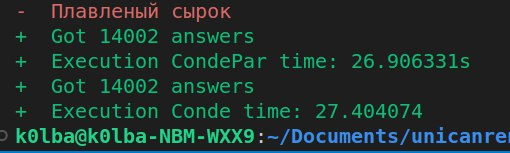
\includegraphics[width=0.8\linewidth]{1test.jpg}
  
  \caption{Входные данные: Параллельно запущены 2 append$^o$ на списках длины 7000 каждый.
  Количество потоков: 2}
  
  \label{fig:mpr}
  
\end{figure}
\begin{figure}[h]

  \centering
    
  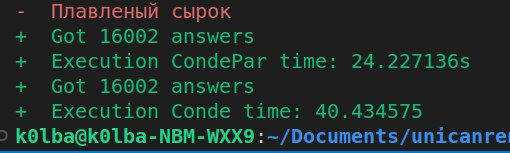
\includegraphics[width=0.8\linewidth]{2test.jpg}
    
  \caption{Входные данные: Параллельно запущены 2 append$^o$ на списках длины 8000 каждый.
  Количество потоков: 12}
    
  \label{fig:mpr}
    
\end{figure}

После нескольких экспериментов, сделан вывод, что запускать при малом количестве потоков, а также на малых обьемах данных не так выгодно, но при росте количества потоков пользы заметно больше.

В результате проведенных тестов я обнаружил, что моя реализация работает не идеально. Если запускать программу, которая рекурсивно вызывает более 70 унификаций, то компилятор выдает ошибку: Task.run.loop
В дальнейших планах доработать эту неисправность и сделать рефакторинг существуюшей реализации
% \begin{enumerate}
% \item Реализация должна быть. На публично доступную реализацию обязательная ссылка. Если код под \textsc{NDA}, то об этом, во-первых, должно быть сказано явно, и, во-вторых, на защиту должны выноситься другие результаты (например, архитектура), чтобы комиссия имела возможность оценить хоть что-то.
% \begin{itemize}
% \item  Рецензент обязан оценить код (о возможности должен побеспокоиться обучающийся).
% \end{itemize} 
% \item Код реализации должен быть написан защищающимся целиком.
% \begin{itemize}
% \item  Если проект групповой, то нужно явно выделить какие части были модифицированы защищающимся. Например, в предыдущих разделах на картинке архитектуры нужно выделить цветом то, что вы модифицировали.
% \item Нельзя пускать в негрупповой проект коммиты от других людей, или людей не похожих на Вас. Например, в 2022 году защищающийся-парень делал коммиты от сценического псевдонима, который намекает на женский ``гендер''. (Нет, это не шутка.) На тот момент в российской культуре это выглядело странно.
% \item Возможна ситуация, что вы используете конкретный ник в интернете уже лет пять, и желаете писать ВКР под этим ником на \GitHub{}. В принципе, это допустимо (не только лишь я так считаю), но если Вы встретите преподавателя, который считает наоборот, то Вам придется грамотно отмазываться. В Вашу пользу могут сыграть те факты, что к нику на гитхабе у Вас приписаны настоящие имя и фамилия; что в репозитории у вас видна домашка за 1й курс; и что Ваш преподаватель практики сможет подтвердить, что Вы уже несколько лет используете это ник; и т.п.
% \end{itemize} 
% \item Если вы получаете диплом о присвоении звания программного инженера, код должен соответствовать. 
% \begin{enumerate}
% \item Не стоит выкладывать код одним коммитом.
% \item Лучше хоть какие-то тесты, чем совсем без них. В идеале нужно предъявлять процент покрытия кода тестами.
% \item Лучше  сделать \textsc{CI}, а также \textsc{CD}, если оно уместно в Вашем проекте.
% \item Не стоит демонстрировать на защите, что Вам даже не пришло в голову напустить на код линтеры и т.п.
% \end{enumerate}
% \item Если ваша реализация по сути является прохождением стандартного туториала, например, по отделению картинок кружек от котиков с помощью машинного обучения, то необходимо срочно сообщить об этом куратору на мат-мехе, иначе Государственная Экзаменационная Комиссия ``порвёт Вас как Тузик грелку'', поставит ``единицу'', а все остальные Ваши сокурсники получат оценку выше. (Это не шутка, а реальная история 2020 года.)
% \item 
% \end{enumerate}

% \noindent Если Вам предстоит защищать учебную практику, а эти рекомендации видятся как более подходящие для защиты ВКР, то ... отмаза не засчитывается, сразу учитесь делать нормально.
\section*{Заключение}
% !TeX spellcheck = ru_RU
% !TEX root = vkr.tex

% \textbf{Обязательно для промежуточного, полугодового, годового и  любых других отчётов.}

В результате работы была реализована параллелизация miniKanren на языке OCaml
Были выполнены поставленные задачи:

% \textbf{Для практик/ВКР.} Также важно сделать список результатов, который будет один к одному соответствовать задачам из раздела~\ref{sec:task}.

\begin{itemize}
\item Выбрана версия Ocaml и библиотека для параллелизации
\item Реализована втроенная параллелизация Unicanren(miniKanren)
\item Проведены тесты и сделан вывод об эффективности реализации
\end{itemize}
% \noindent Для промежуточных отчетов сюда важно записать какие задачи уже были сделаны за осенний семестр, а какие только планируется сделать.

% Также сюда можно писать планы развития работы в будущем, или, если их много, выделять под это отдельную главу.



\setmonofont[Mapping=tex-text]{CMU Typewriter Text}
  \bibliographystyle{ugost2008ls}
  \bibliography{vkr}
\end{document}
